\chapter{Architecture Design}
\label{ch:Architecture Design}

\section{Proposed Architecture}

This section describes the overall architecture of the project shown in the figure {Ref} . The SCrAMbLE software suite comprises of a Translator, a Splitter and an Adaptor as its modules.

The software suite has a main engine which facilitates interoperability between these modules established with different docker containers. The whole suite is again managed inside a docker container by the main engine. Communication between the MANO frameworks and the SCrAMbLE software suite is achieved through plugins which are intergrated inside the MANOs, in the form of HTTP requests.

Upon receiving a service request from a MANO through the REST calls, the main engine identifys the type of service request and channels the request to the appropriate modules, with the help of a message broker , RabbitMQ.

The main engine uses nameko services to manage REST calls and RabbitMQ message broker. It also collects results from service modules or the service completion information, and send it to the MANO framework. The engine also uses MongoDB database to store and retrieve the intermediate and result information like NSD, VNFD files.


The workflow of the individual service modules is explained in the sections below.


\begin{figure}[H]
	\centering
	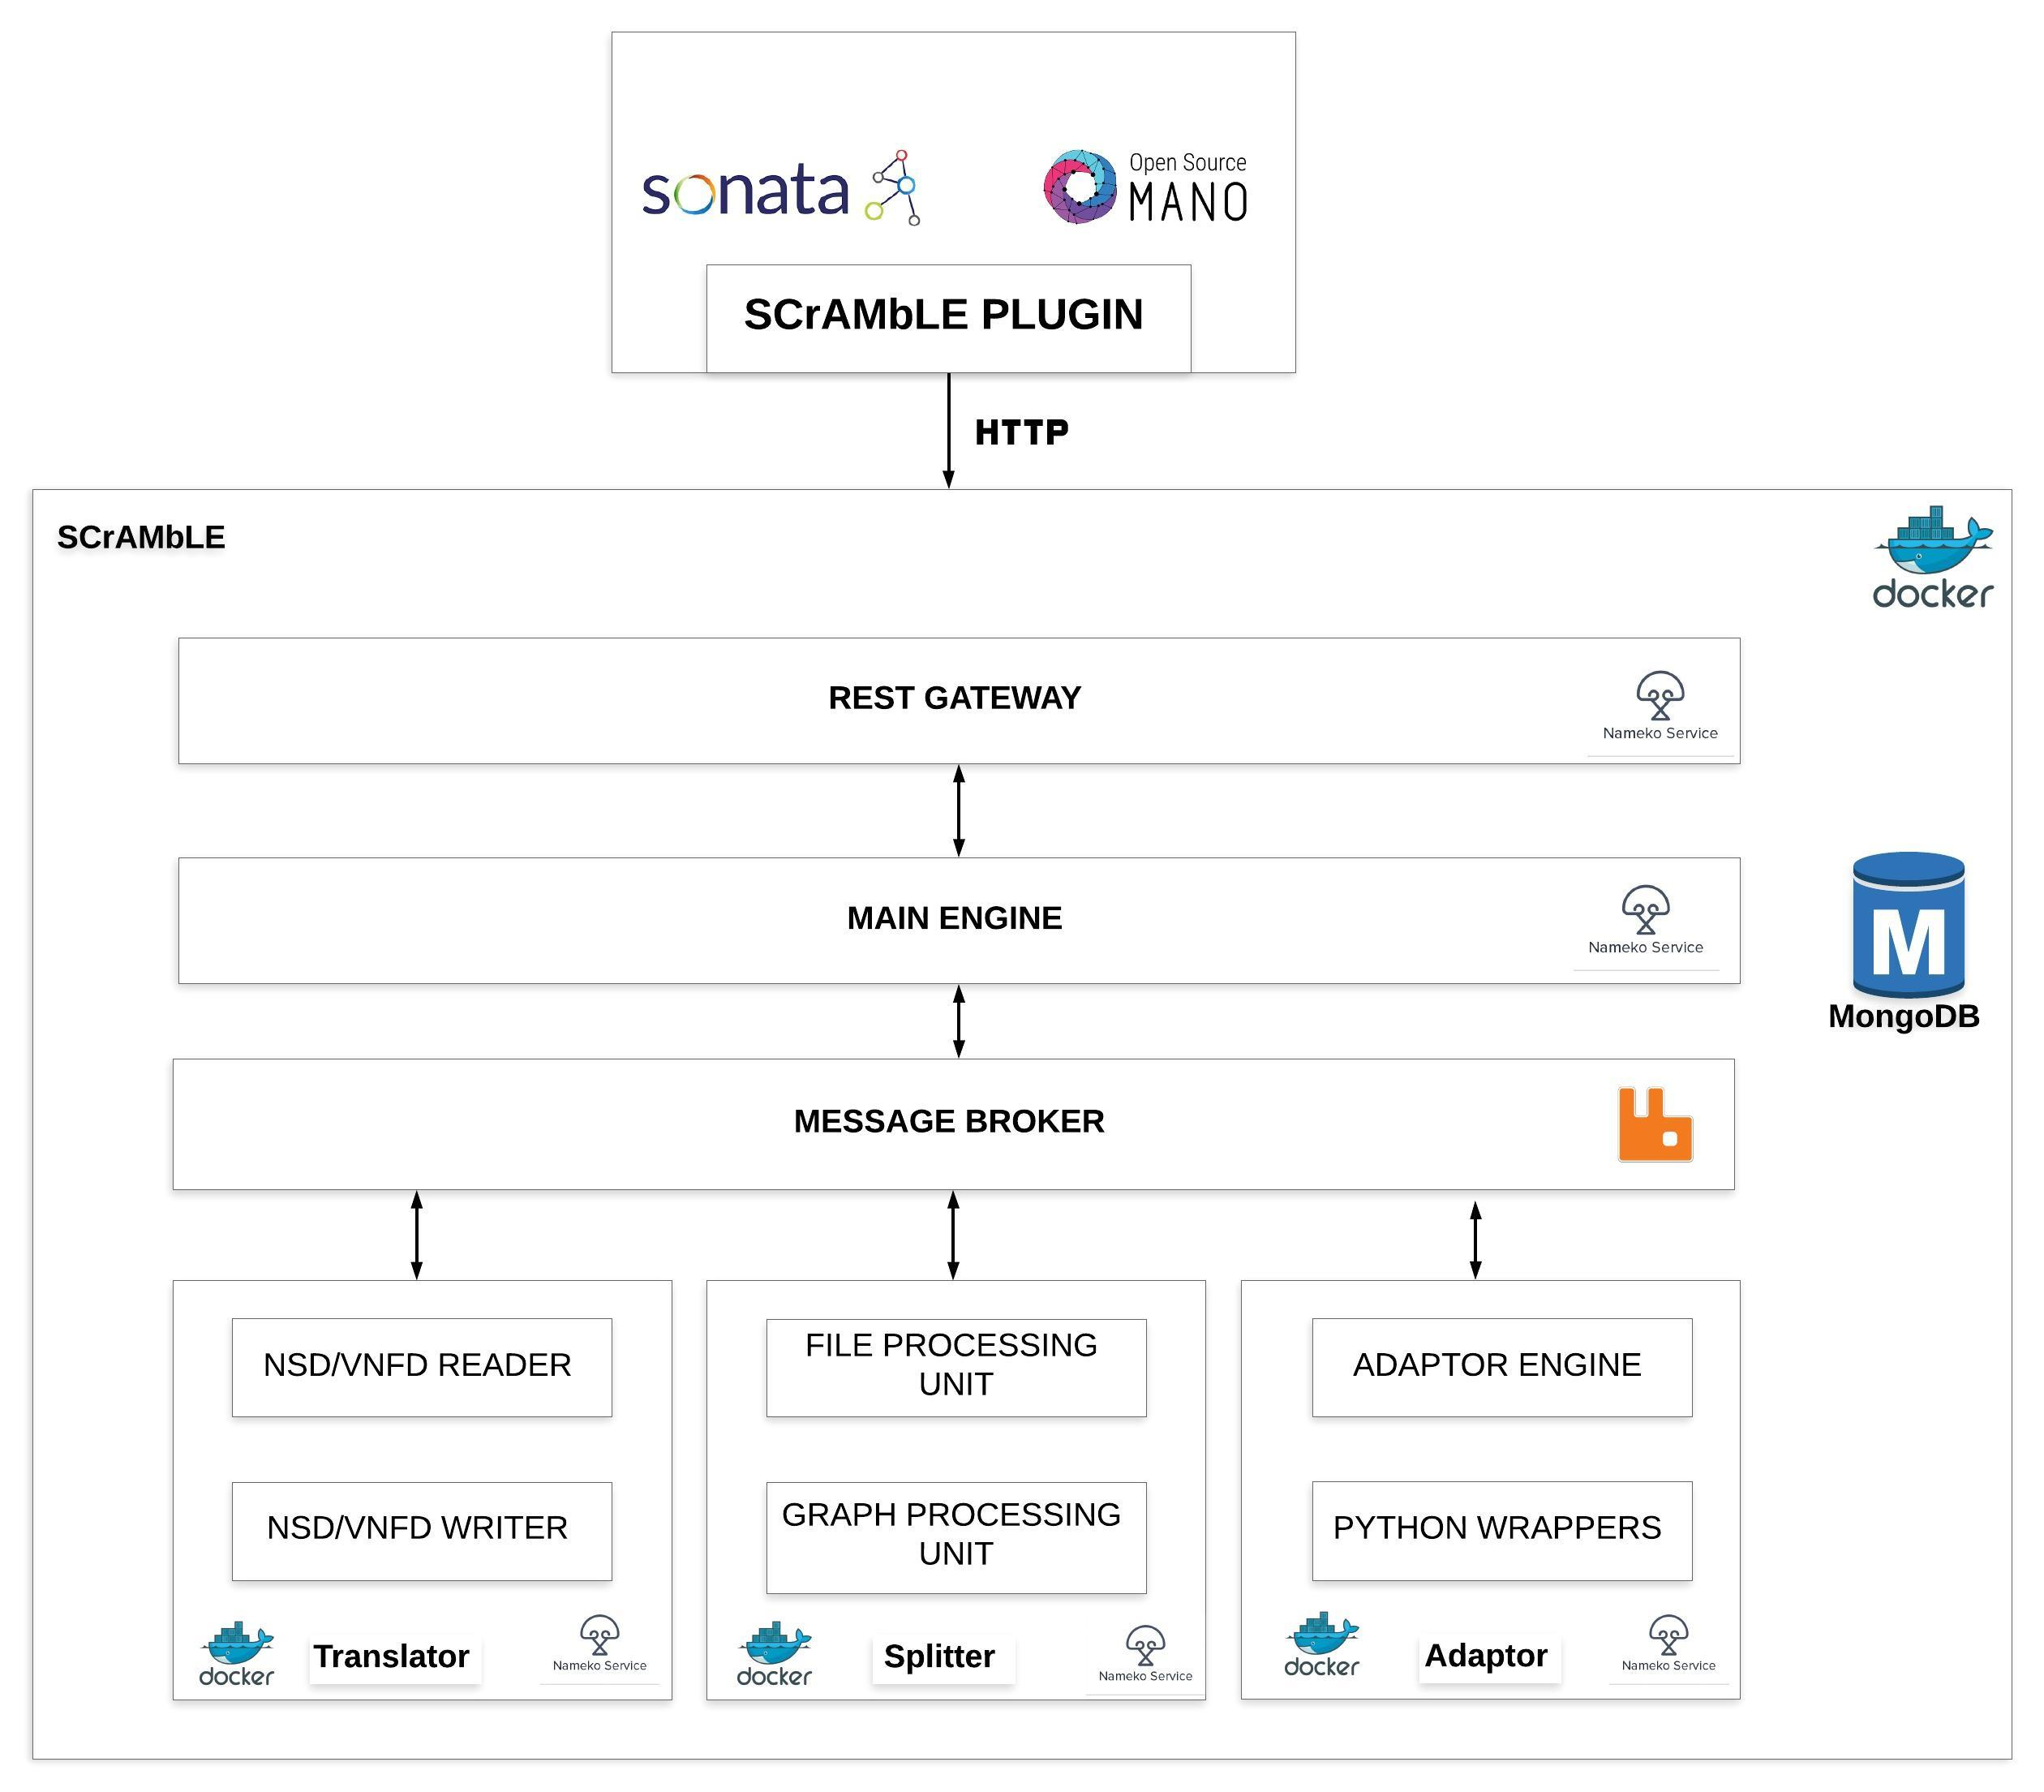
\includegraphics[width=0.9\linewidth]{figures/Scramble_Architecture}
	\caption{Project reference architecture}
	\label{fig:Scramble_Architecture}
\end{figure}

\subsection{Adaptor Workflow}

\subsection{Service Descriptor Splitter Workflow}

\subsection{Service Descriptor Translator Workflow}
In a scenario where a network service is to be deployed among different MANO frameworks, having their own respective schema, SDT translates a NSD schema of one MANO framework to that of other MANO framework.

On receiving a service request to translate a NSD and/or VNFD to schema of a different MANO, the main engine stores the file(s) into the MongoDB as a document and sends a request in the form of a message to SDT usinfg Nameko services. The message contains the information of DB document name and document id, source type and destination type. 

SDT comprises of two main services, namely, a Reader and a Writer. On receiving the message from main engine, the Reader fetches the file/document from DB and validates it. After validating the file will be converted to intermediate format, which will be sent to Writer. The Writer converts the file from intermediate format to the destination file format mentioned in the request. On completion of translation, the translated file will be stored into MongoDB and the reference to the same will be passed to main engine with the service completion message.

This is an overview of the workflow for Service Descriptor Translator. The details of the message parameters communication between the components are subjected to changes in development phase.


\begin{figure}[H]
	\centering
	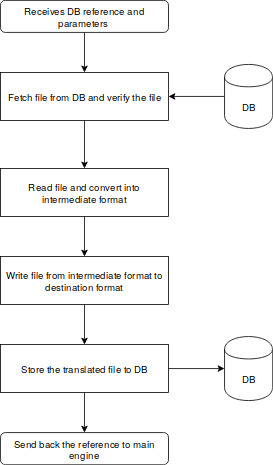
\includegraphics[width=0.5\linewidth]{figures/SDT_Workflow}
	\caption{Service Descriptor Translator Workflow}
	\label{fig:SDT Workflow}
\end{figure}

   





